\section{Data Analysis of Study}
Table for number of points per day per participant etc
The number of valid days for a specific feature is a day for which the user gave answers, and the feature could be calculated. If the user for example turned off their phone during the night, the home stay feature could not be calculated, but the routine index feature and the number of places will likely still have been calculated.

\begin{figure}
    \centering
    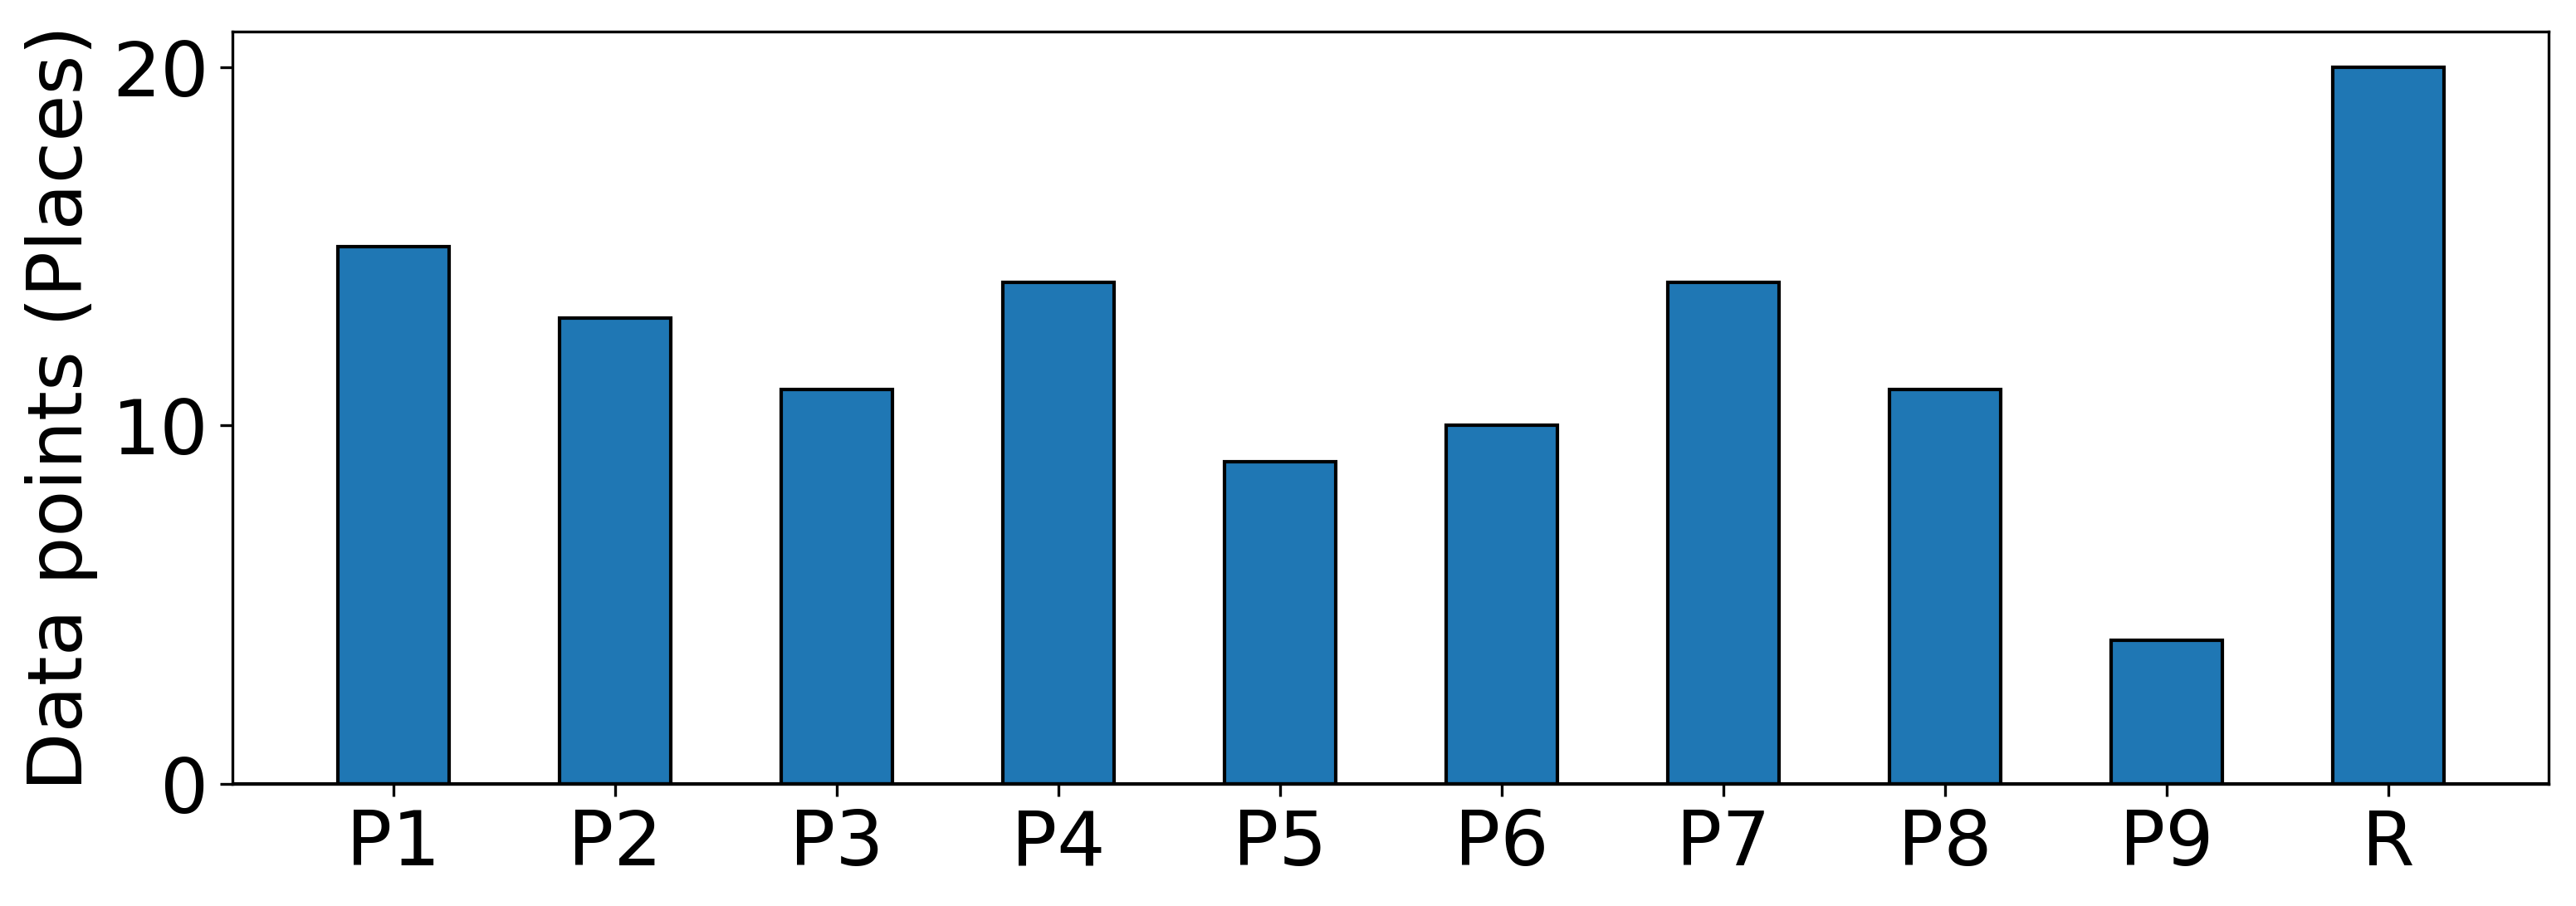
\includegraphics[0.5\textwidth]{images/study/n_places.png}
    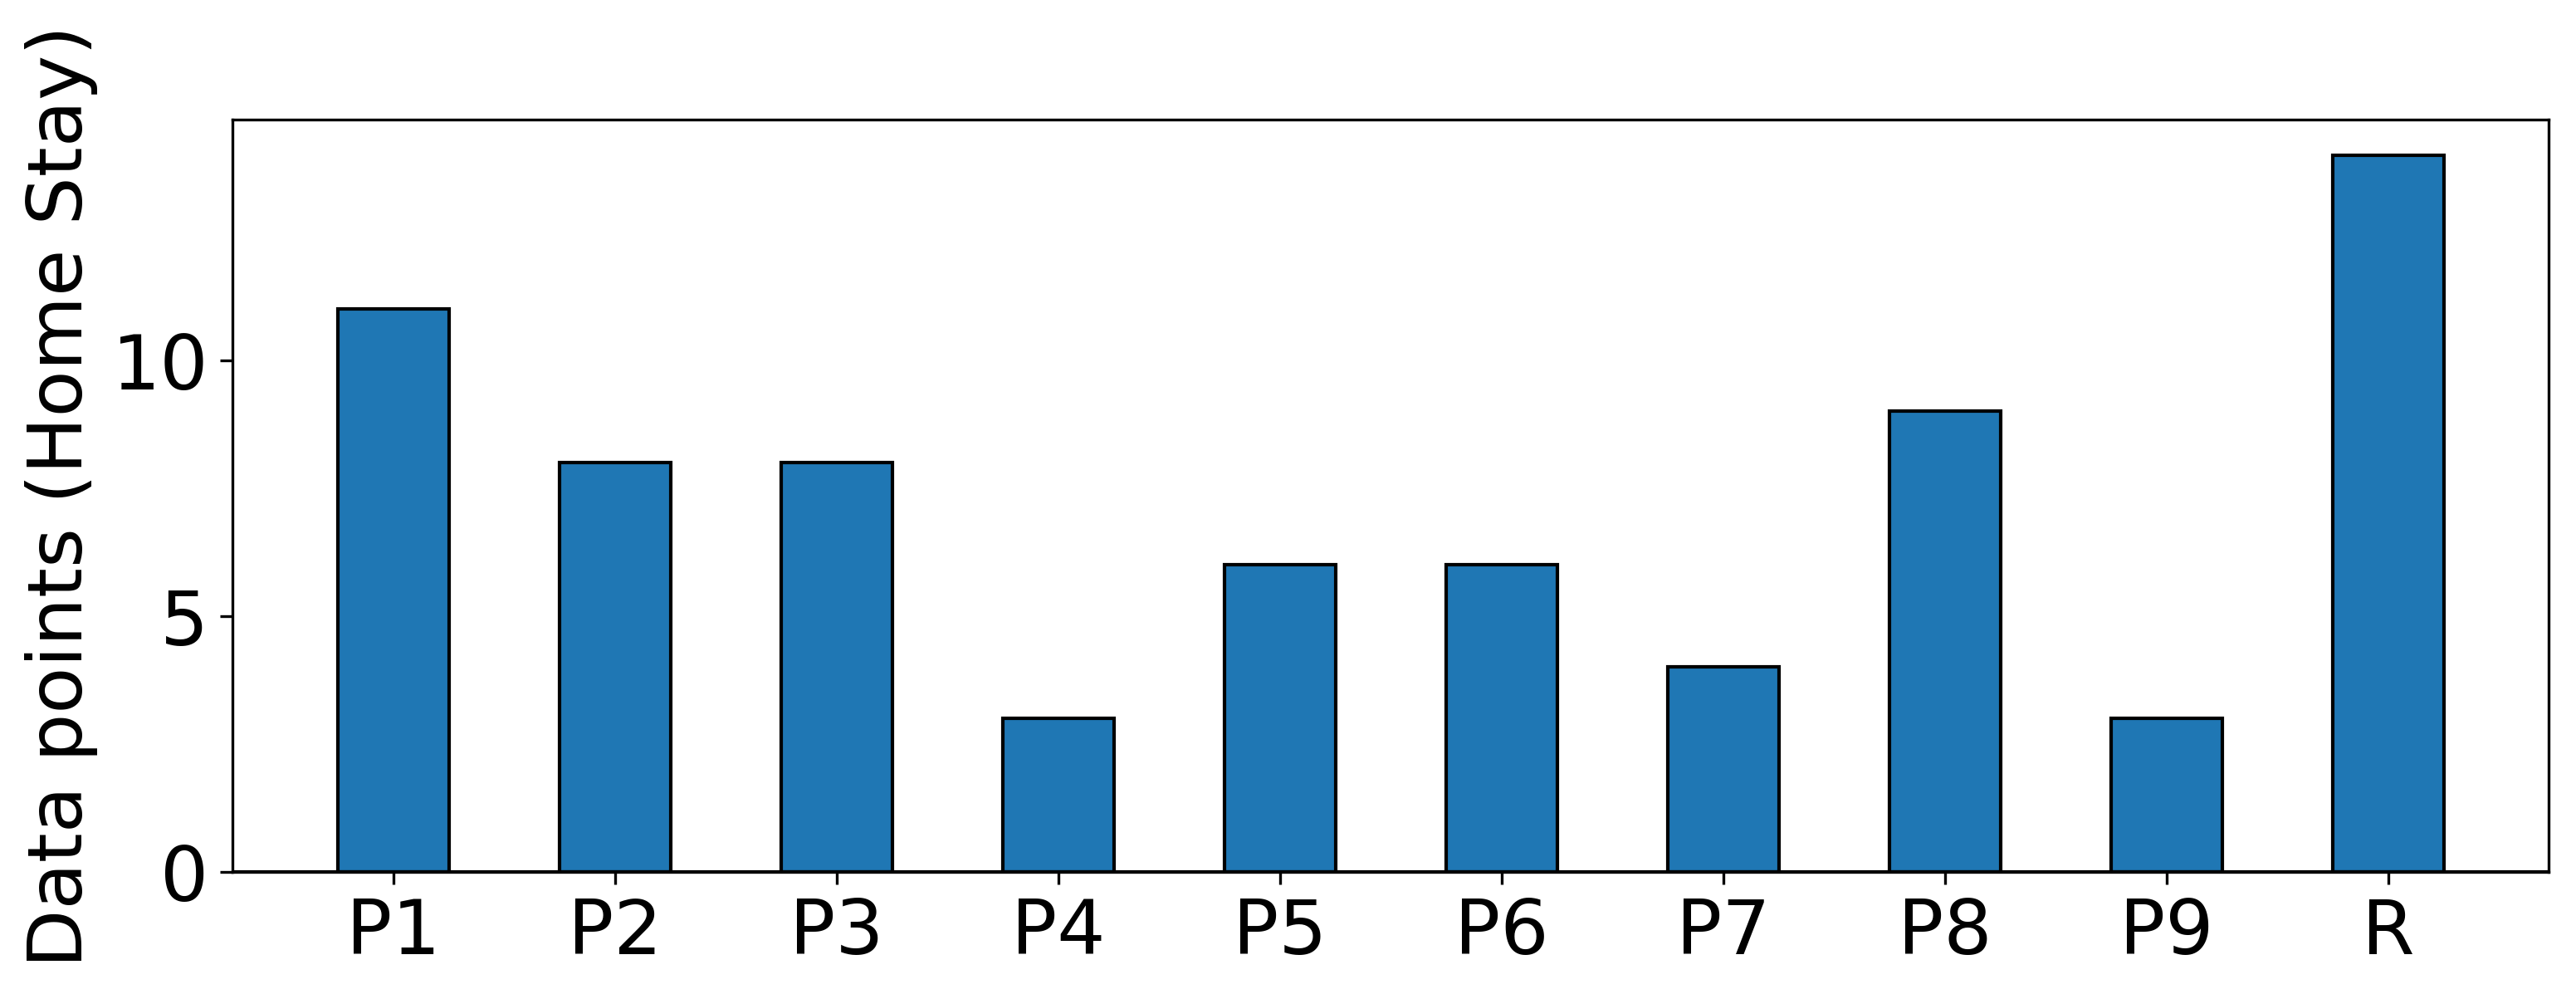
\includegraphics[0.5\textwidth]{images/study/n_homestay.png}
    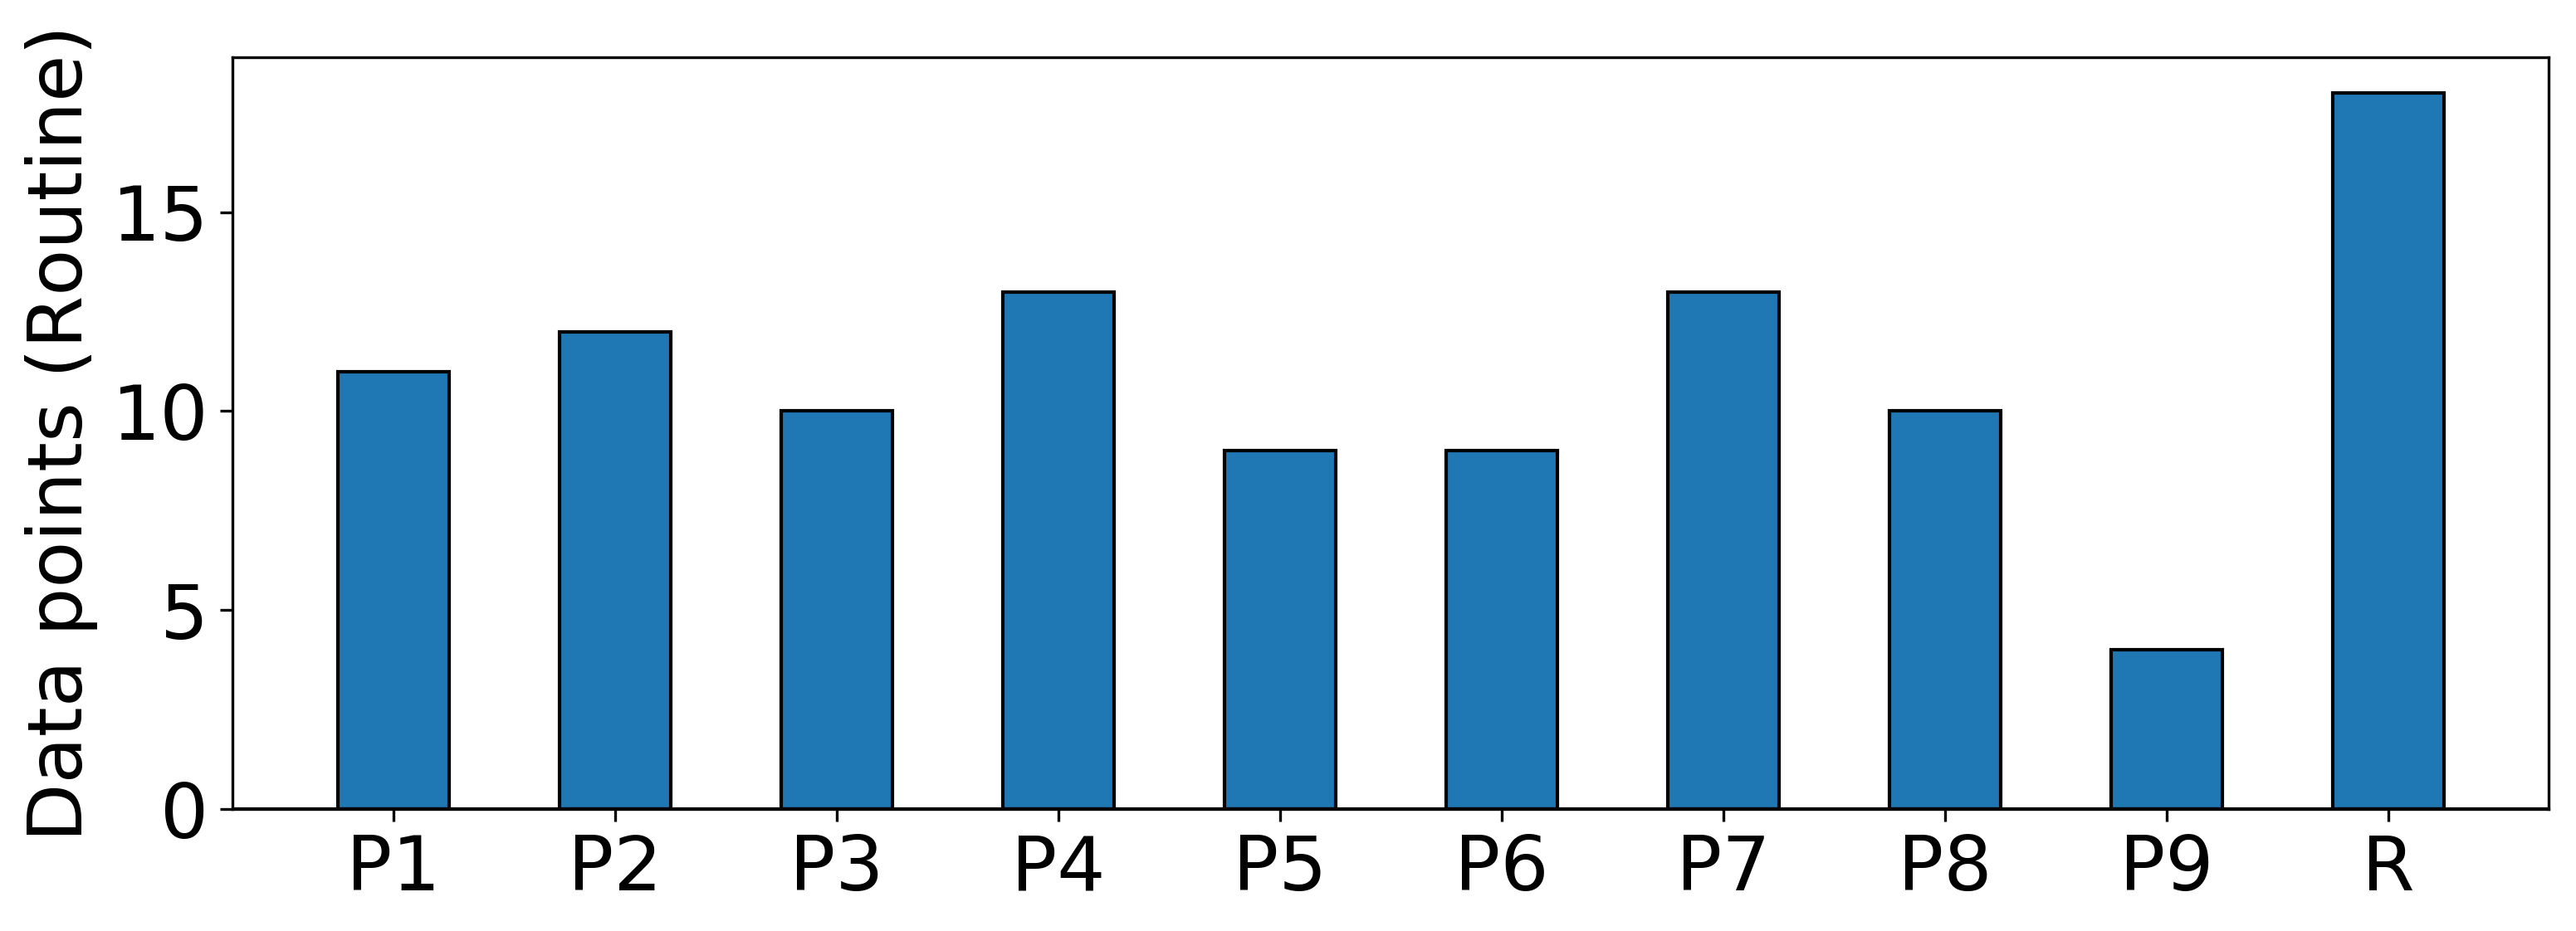
\includegraphics[0.5\textwidth]{images/study/n_routine.png}
    \caption{The number of valid days for each participant}
    \label{fig:plot-daily}
\end{figure}

The day-by-day results for the author are displayed in figure \ref{fig:plot-daily}.

\begin{figure}
    \centering
    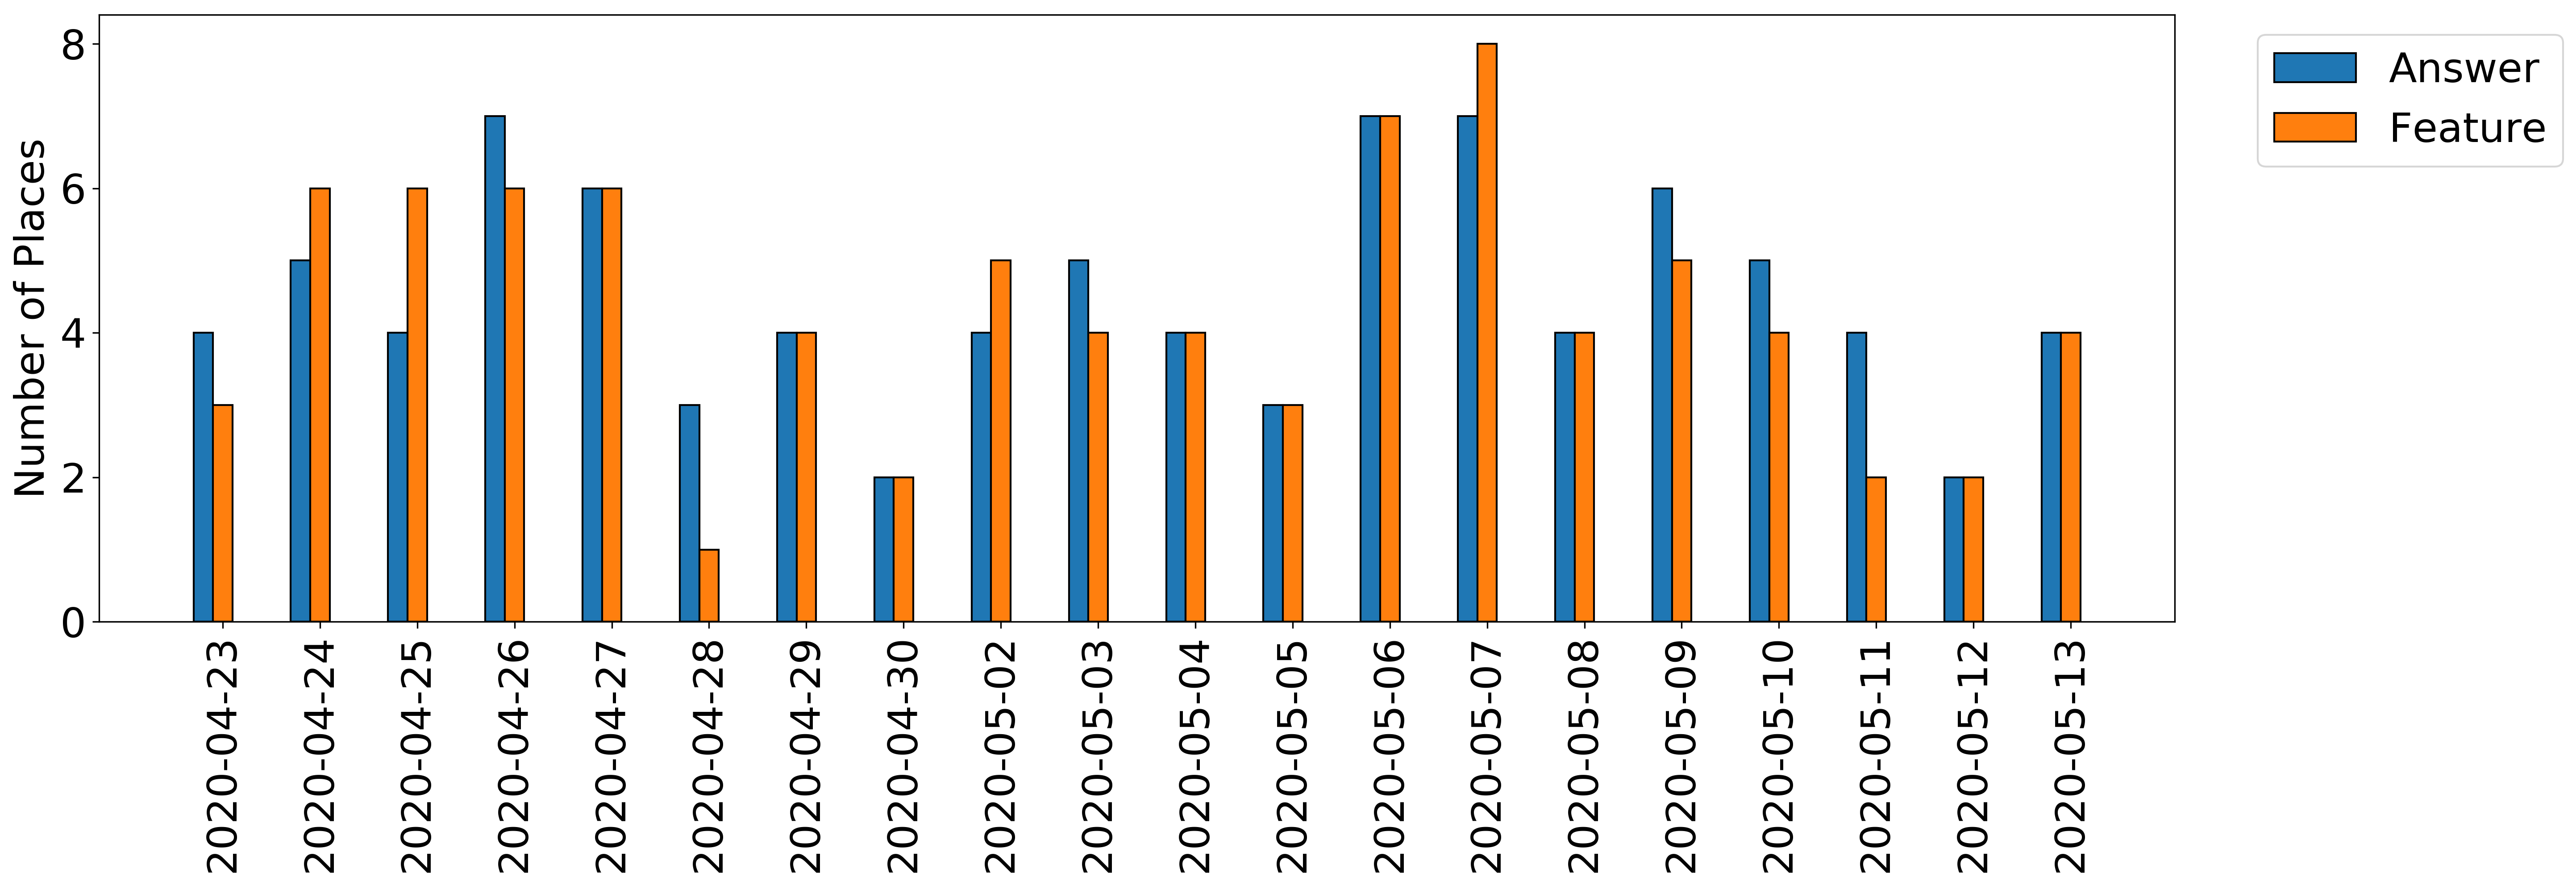
\includegraphics[0.5\textwidth]{images/study/places_d6b2d9b9-398b-4e0d-b52b-224747f515c8.png}
    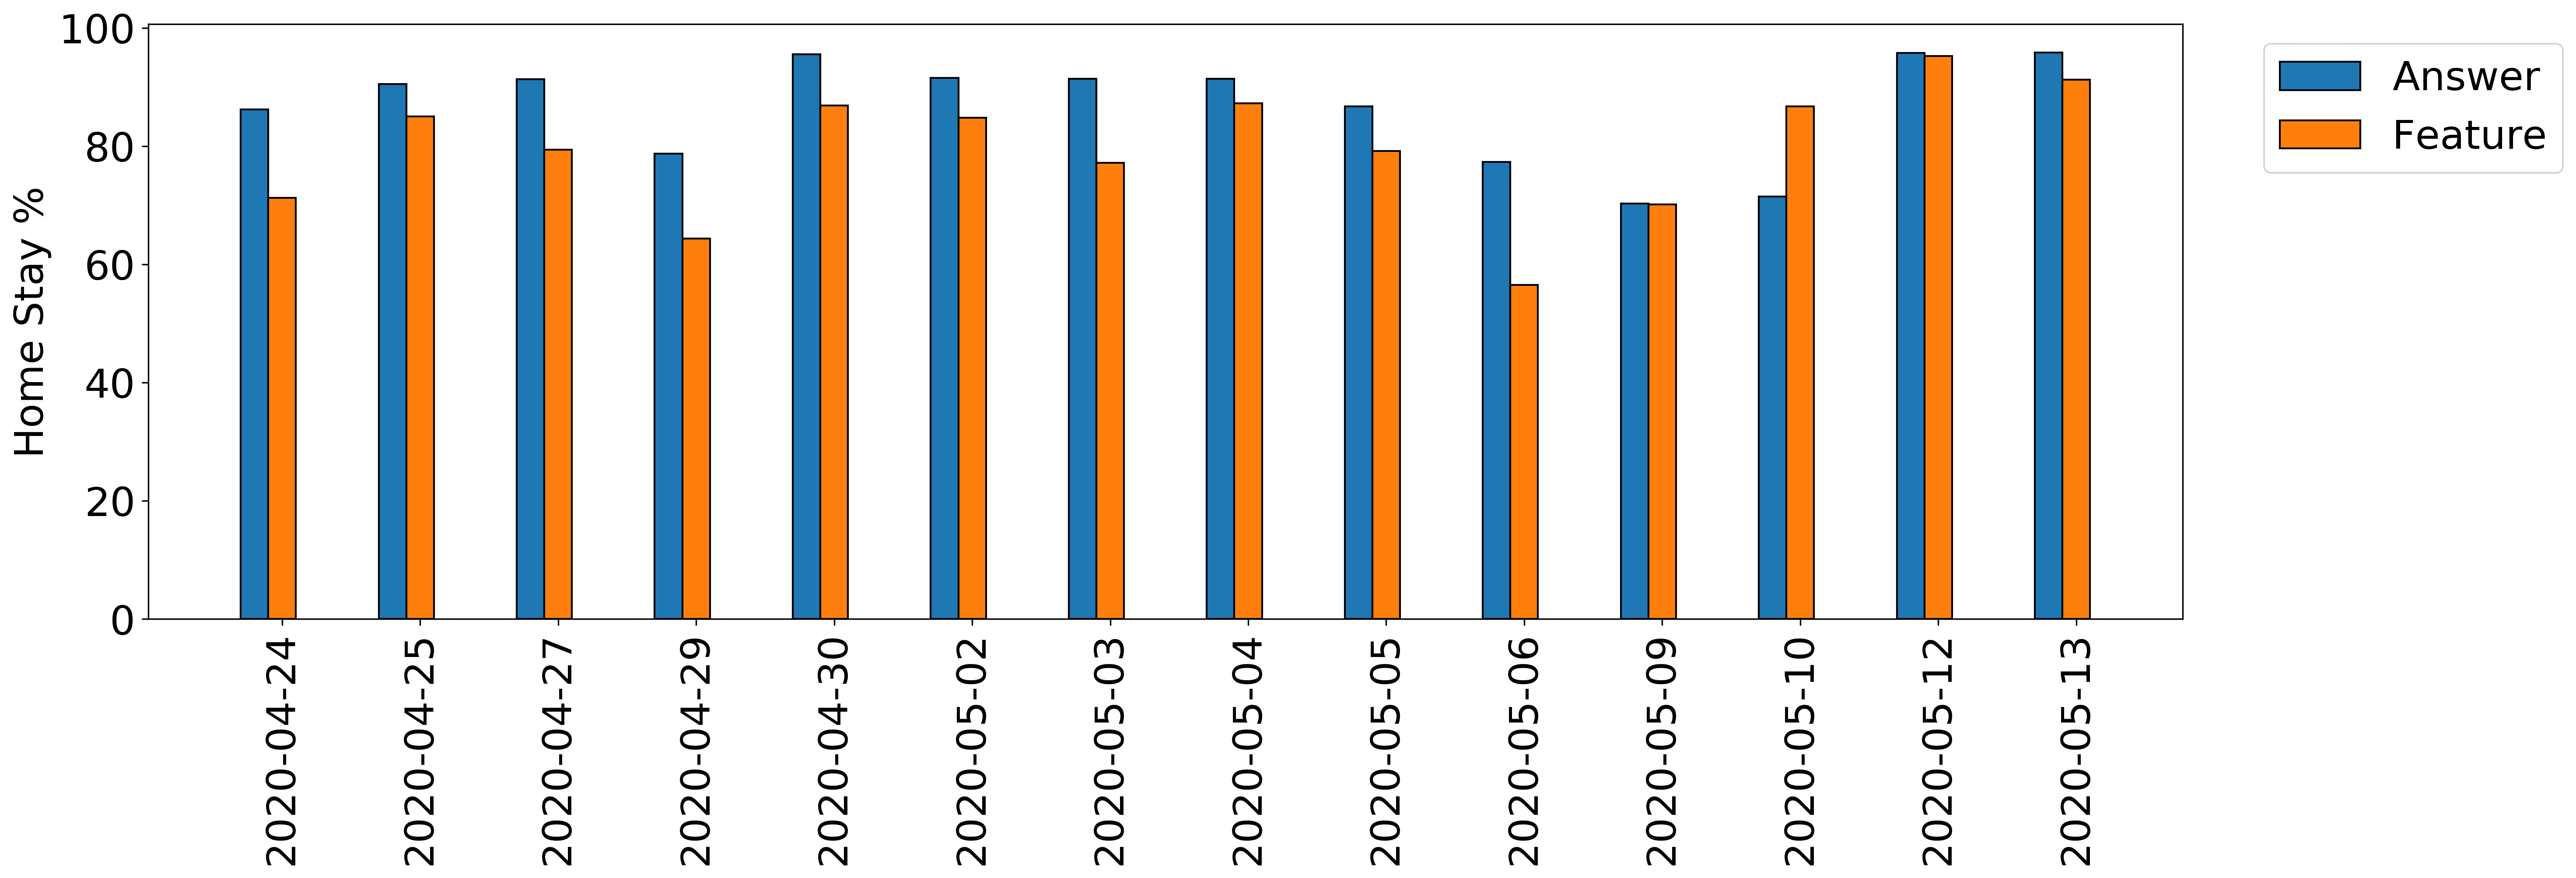
\includegraphics[0.5\textwidth]{images/study/homestay_d6b2d9b9-398b-4e0d-b52b-224747f515c8.png}
    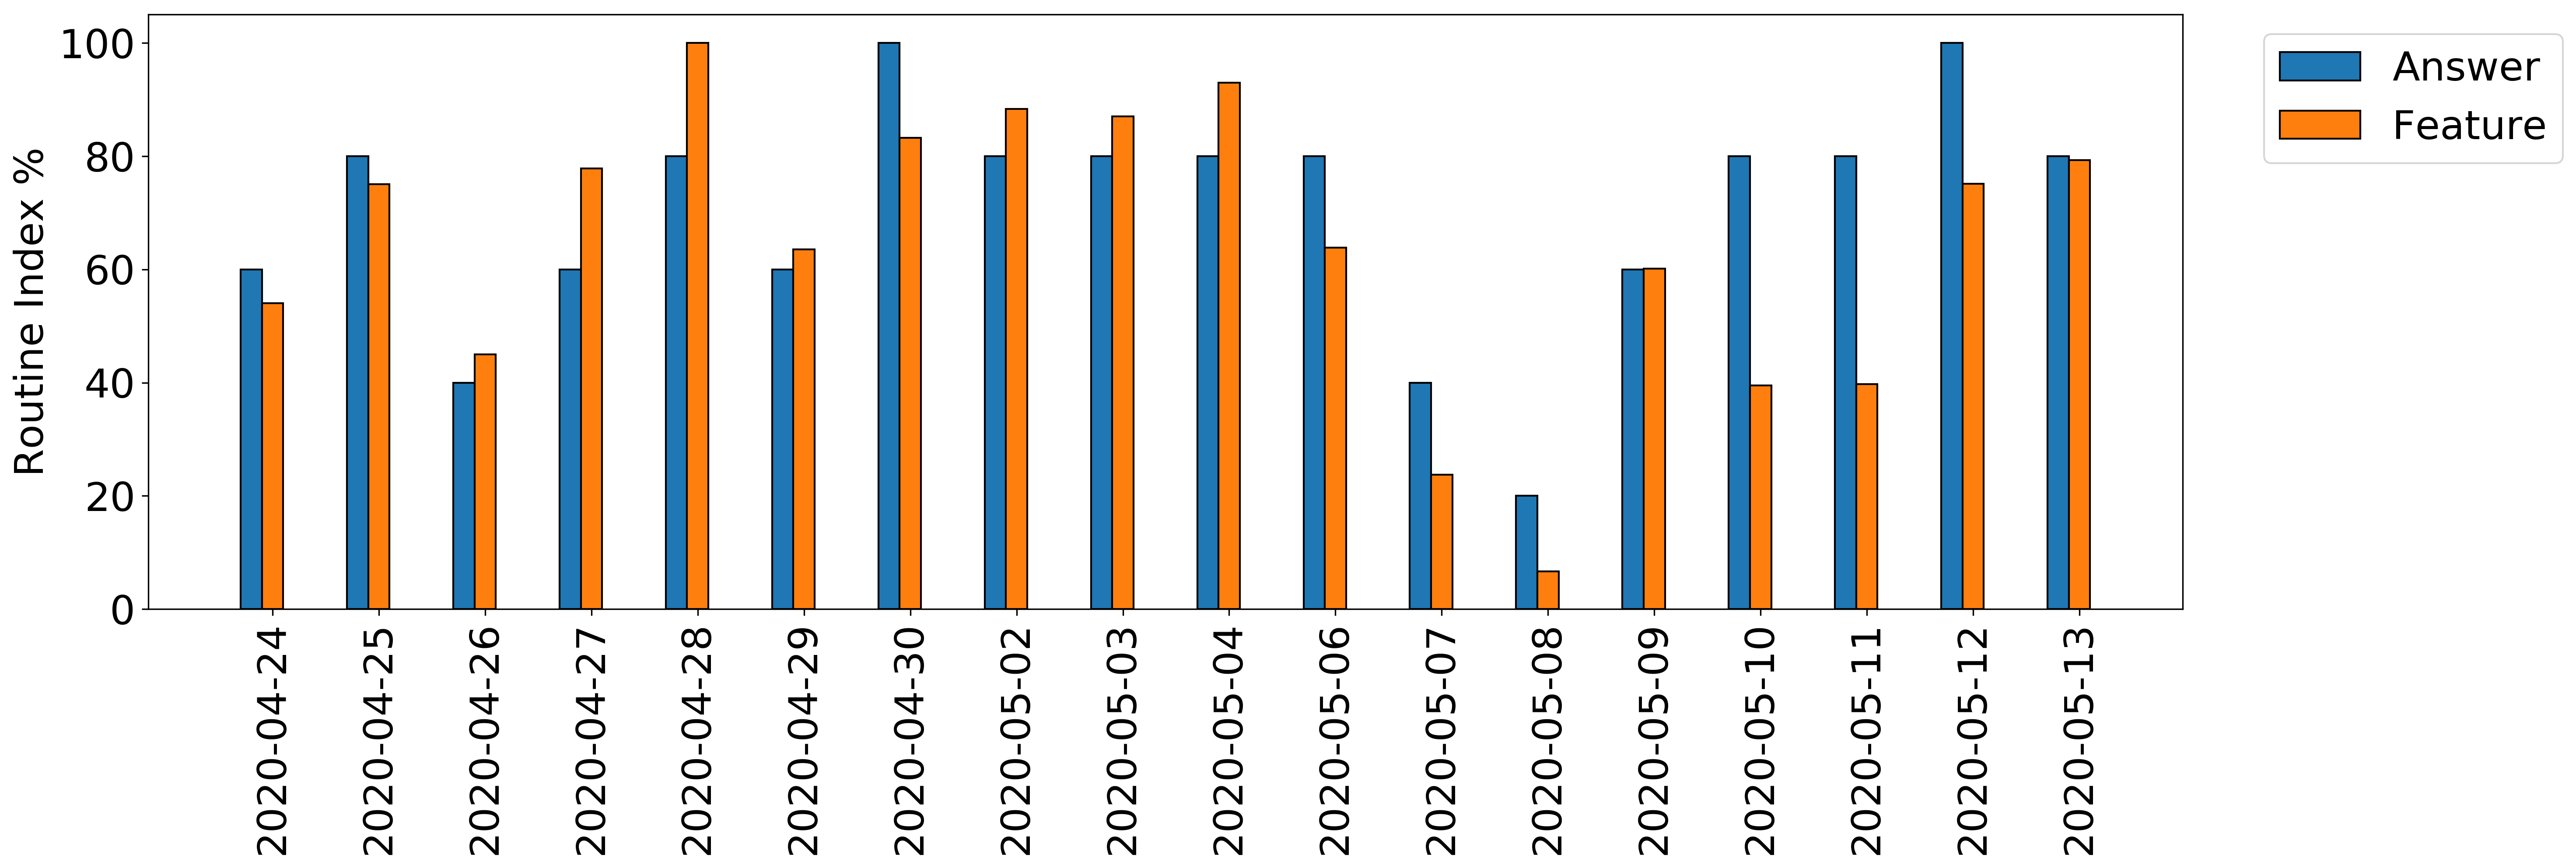
\includegraphics[0.5\textwidth]{images/study/routine_d6b2d9b9-398b-4e0d-b52b-224747f515c8.png}
    \caption{The answered and calculated data for each day, for the author}
    \label{fig:plot-daily}
\end{figure}

To say something about whether or not the algorithms undershoots or overshoots, the difference in sum was calculated as $E = \frac{\sum(A) - \sum(F)}{N}$ ($N$ being the total number of days for the specific feature) meaning that if the result is positive then the answered result was on average higher and vice versa if the result is negative. 

\begin{figure}
    \centering
    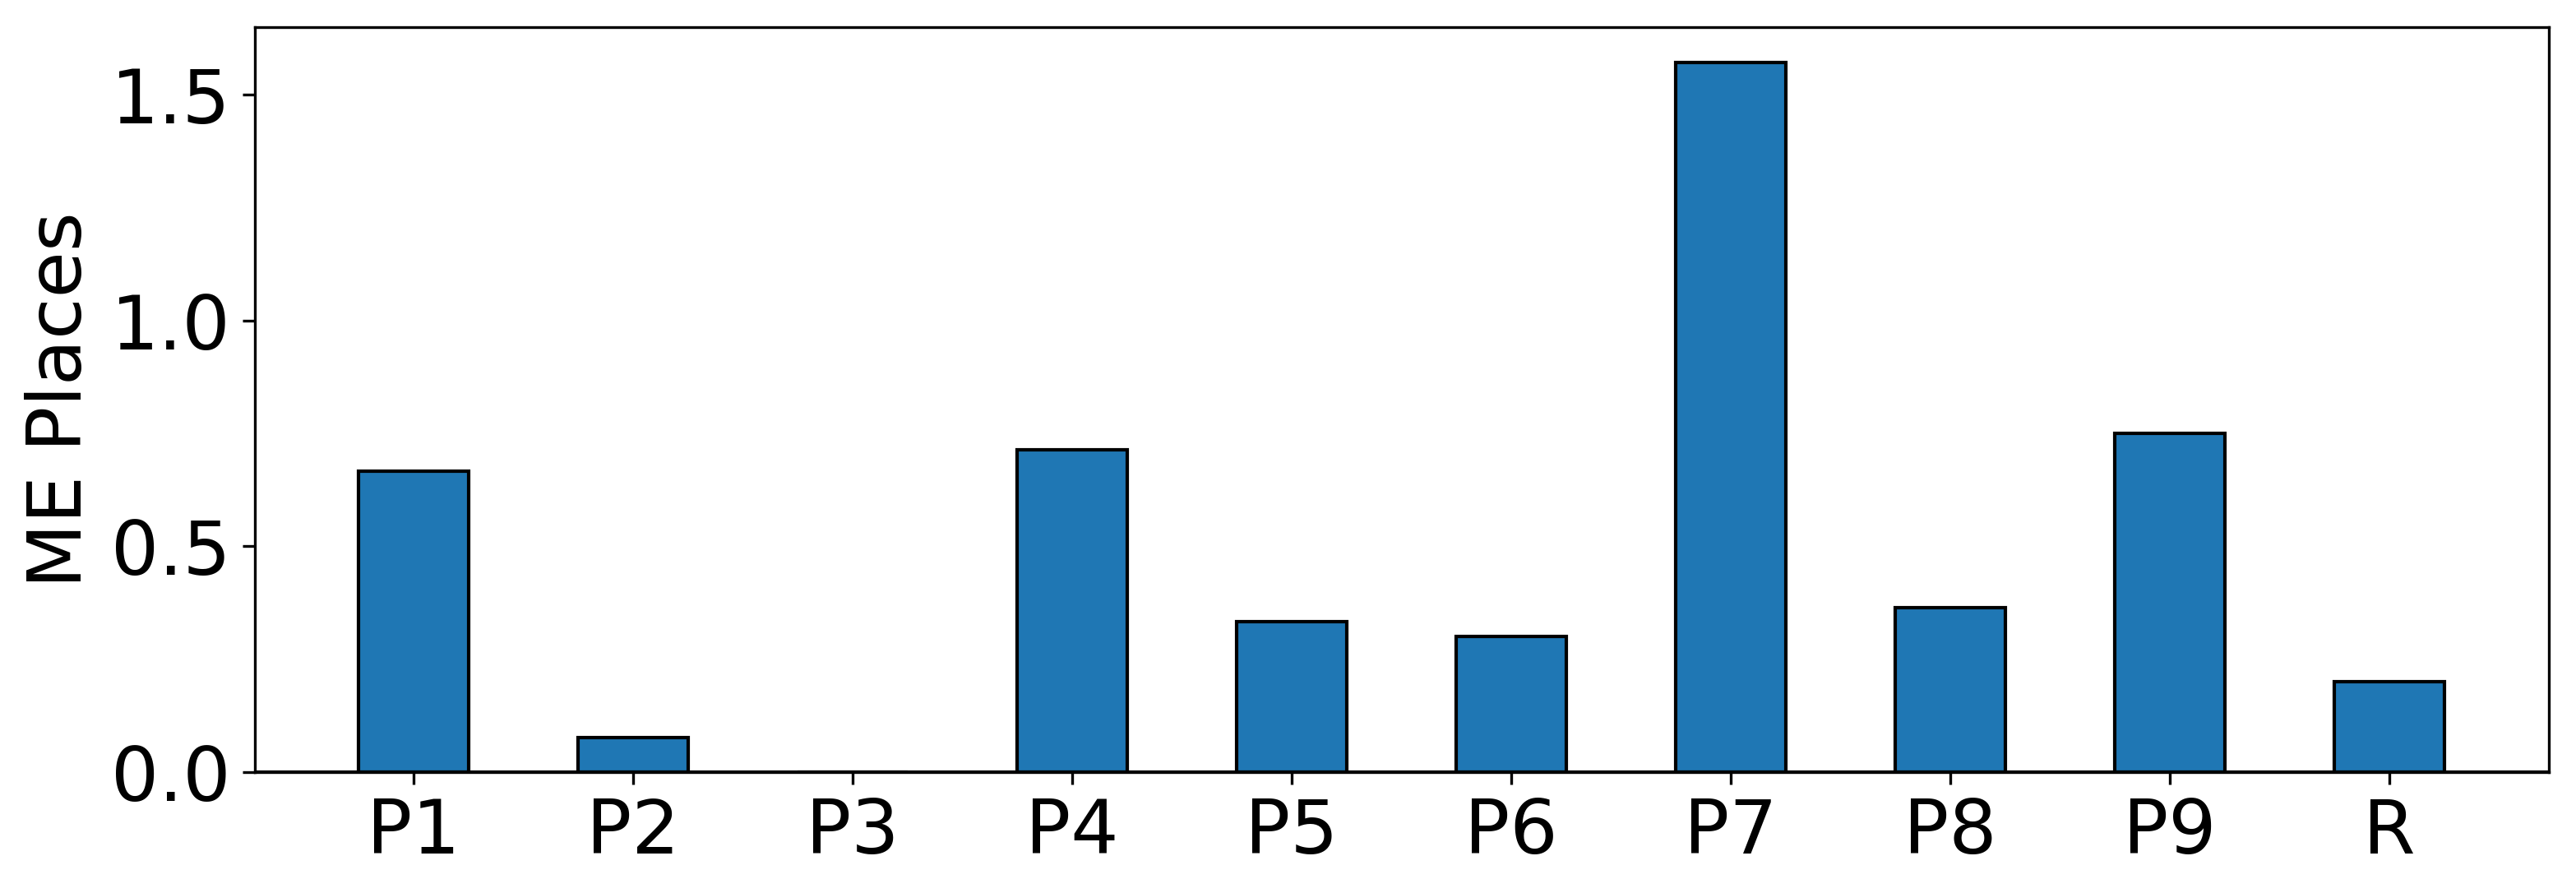
\includegraphics[0.5\textwidth]{images/study/me_places.png}
    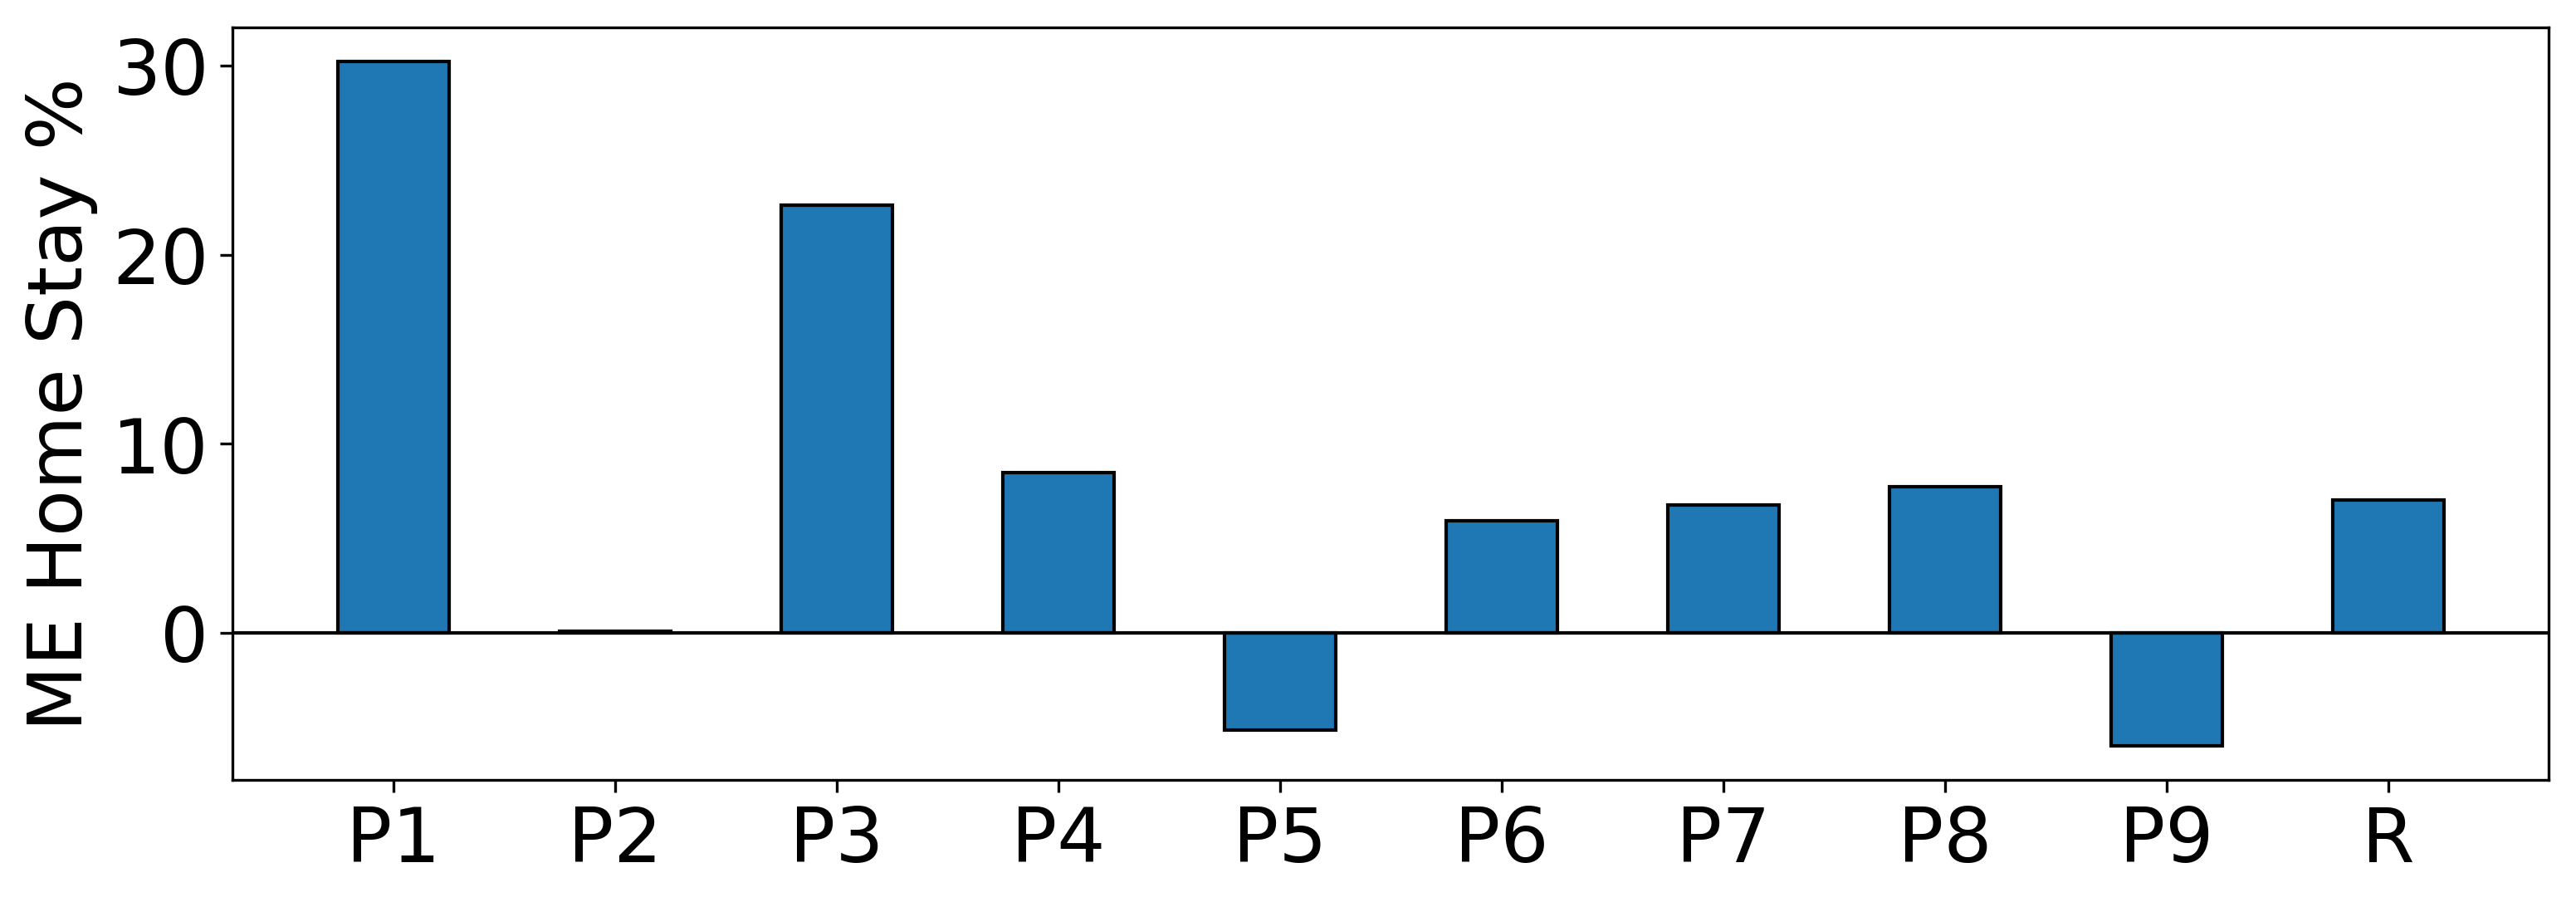
\includegraphics[0.5\textwidth]{images/study/me_homestay.png}
    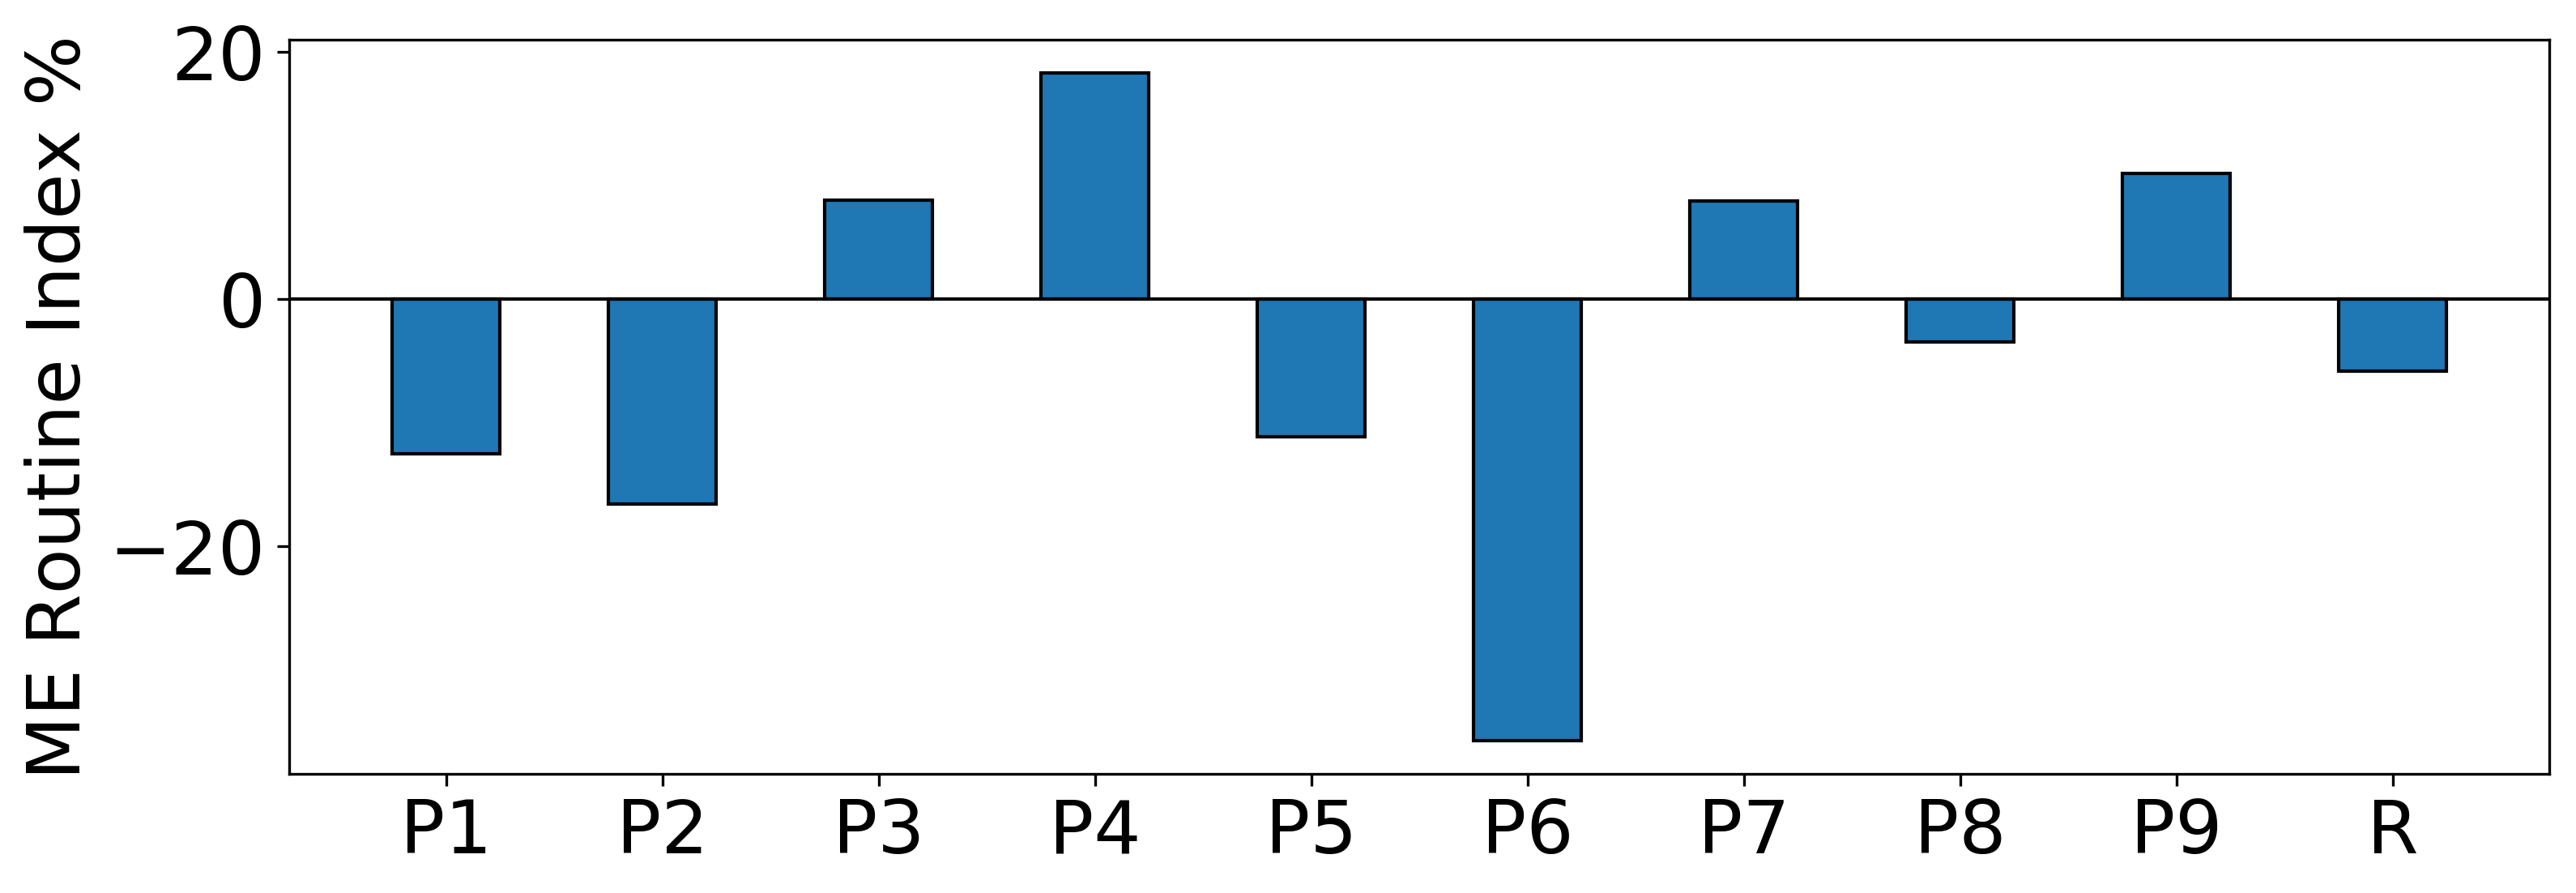
\includegraphics[0.5\textwidth]{images/study/me_routine.png}
    \caption{The number of data points in terms of days which could be evaluated, for each participant}
    \label{fig:plot-mean-error}
\end{figure}

errors and accuracy 
Participant answers are not ground truth
Its better to consistently under-shoot, that to oscillate
Registering during the night
home stay undershoots often